
\section*{Energy Calibration}

Due to the organic composition of our detectors the photo-electric cross-section of its constituents is negligible in the energy range considered. Furthermore total absorption through multiple Compton scattering is negligible too, because of detector limited size . The detectors response will be dominated by individual Compton interaction, thus the energy spectrum is a continuous distribution that corresponds to different angles of interaction. This can be seen in the spectra acquired with the $^{22}$Na source in Fig. \ref{fig: uncalibrated energy spectra}.

\smallskip
\begin{figure}[h!]
\centering
\subfloat[][\emph{Detector 1 }.]
   {\includegraphics[width=.45\textwidth]{d1_spectrum_qlong}} \quad
\subfloat[][\emph{Detector 2 }.]
   {\includegraphics[width=.45\textwidth]{d2_spectrum_qlong}} \\
\caption{\emph{Detector 1} (a) and \emph{Detector 2} (b) uncalibrated energy spectra  obtained from a $^{22}$Na $\gamma$ source.}
\label{fig: uncalibrated energy spectra}
\end{figure}

The finite resolution of our detectors result in a shift towards lower energies depending on the detector resolution as shown in Fig.~\ref{fig: smeared spectra}.
\begin{figure}[h!]
\centering
\includegraphics[width=0.8\textwidth]{smeared_spectra}
\caption{Gaussian smeared spectra at different $\sigma$ generated using the  Klein-Nishina Compton Scattering cross-section  for 511~keV photons.}
\label{fig: smeared spectra}
\end{figure}

In order to obtain the energy calibration parameters, several smeared spectra were generated using the  Klein-Nishina Compton Scattering cross-section~(see Eq.~\ref{eq:Klein-Nishina}) for $511$ keV and $1275$ keV $\gamma$ respectively.
\begin{equation}
\dfrac{d\sigma}{dT} = \dfrac{\pi r_e^2}{m_ec^2\alpha^2}\left(2+\dfrac{s^2}{\alpha^2(1-s)^2}+\dfrac{s}{1-s} \left(s-\dfrac{2}{\alpha}\right) \right)
\label{eq:Klein-Nishina}
\end{equation}
To locate the Compton edge then, the background from acquired spectra was removed  as shown in Fig.~\ref{fig: compton back}.
\begin{figure}[h!]
\centering
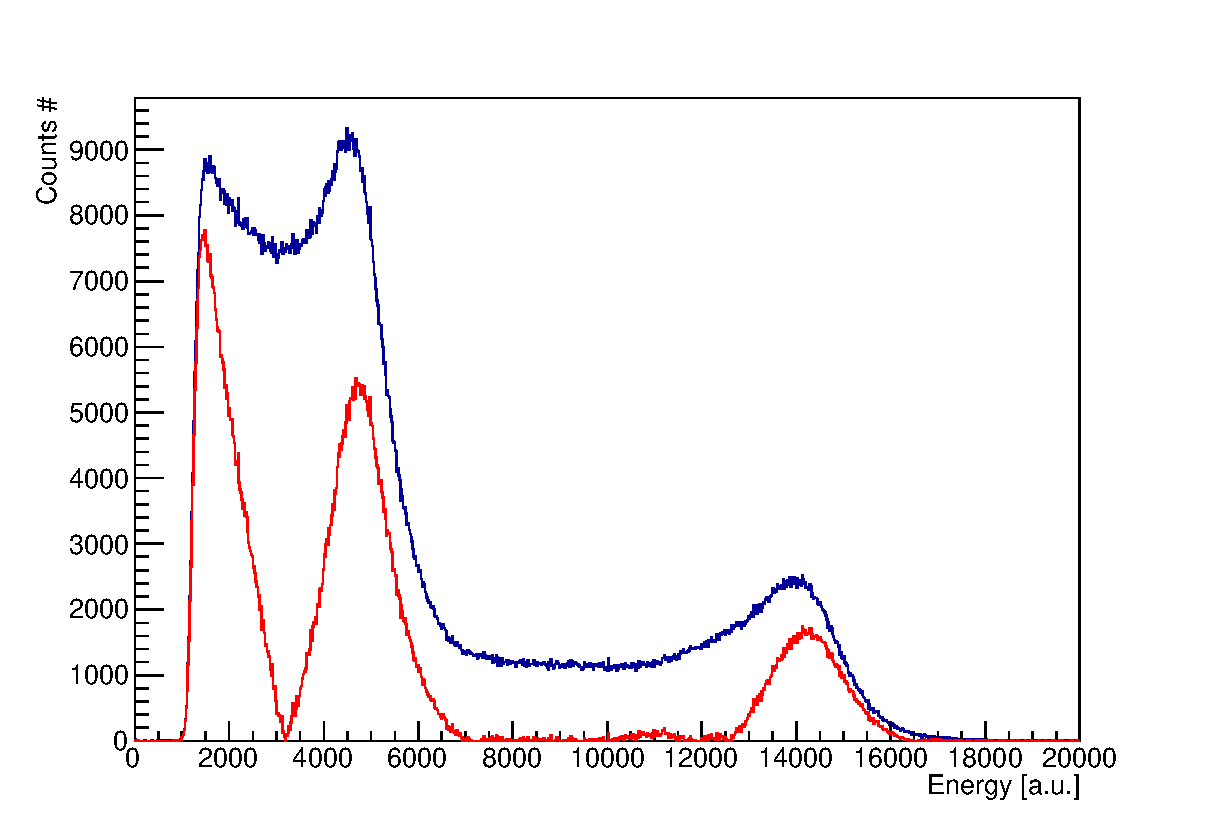
\includegraphics[width=0.8\textwidth]{spectra_vs_background.eps}
\caption{$^{22}$Na energy spectra. The blue one represent the original acquired spectrum, while the red one is obtained by background removal.}
\label{fig: compton back}
\end{figure}
%%%%%%%%%%%%%%%%%%%%%%%%%%%%%%%%%%%%%%%%%%5
Once we have the compton edge position we have to loop on every previous generated smearing and calculating the $\chi^2$ between experimental spectrum and gaussian smeared one selecting the smearing with the $\sigma$ that led to minimum $\chi^2$. Once we have selected a proper $\sigma$ we have also the corresponding shift of the Compton Edge that we have to use in order to calibrate our detector.

\begin{figure}[h!]
\centering
\subfloat[][\emph{Detector \#1 spectrum}.]
   {\includegraphics[width=.45\textwidth]{calibrated_spectra_d1}} \quad
\subfloat[][\emph{Detector \#2 spectrum}.]
   {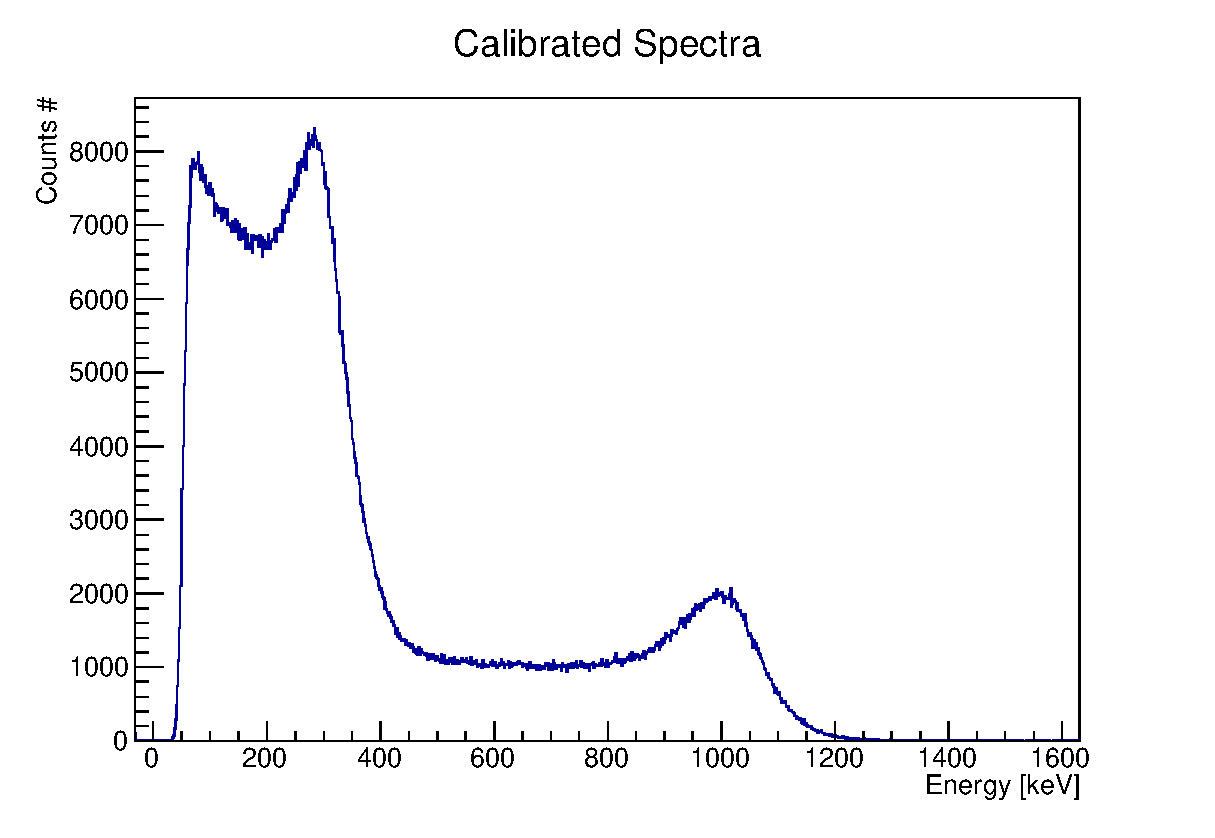
\includegraphics[width=.45\textwidth]{calibrated_spectra_d2}} \\
\caption{Calibrated detectors spectra.}
\label{fig: calibrated energy spectra}
\end{figure}

\begin{table}[h!]
\centering
\begin{tabular}{ccc}
\toprule
\toprule
Photon Energy [keV] & $\sigma$ [keV] & C.E. shifting [keV] \\
\midrule
511 & 34& 40.66 \\
1275 & 40 & 52.15\\
\bottomrule
\bottomrule
\end{tabular}
\caption{$\sigma$ and C.E. shift for detector \#1.}
\end{table}

\begin{table}[h!]
\centering
\begin{tabular}{ccc}
\toprule
\toprule
Photon Energy [keV] & $\sigma$ [keV] & C.E. shifting [keV] \\
\midrule
511 & 28 & 34.66 \\
1275 & 40 & 52.15\\
\bottomrule
\bottomrule
\end{tabular}
\caption{$\sigma$ and C.E. shift for detector \#2.}
\end{table}
\begin{table}[h!]
\centering
\begin{tabular}{ccc}
\toprule
\toprule
Detector & a [keV/channel] & b [keV] \\
\midrule
\#1 &  0.0748945$\pm$ & -54.2511$\pm$ \\
\#2 & 0.083215$\pm$ & -32.6856$\pm$ \\
\bottomrule
\bottomrule
\end{tabular}
\caption{Calibration parameters.}
\end{table}



%\begin{figure}[h!]
%\centering
%\subfloat[][\emph{Low energy Compton Edge}.]
%   {\includegraphics[width=.45\textwidth]{fit_511_d1}} \quad
%\subfloat[][\emph{High energy Compton Edge}.]
%   {\includegraphics[width=.45\textwidth]{fit_1275_d1}} \\
%\caption{Compton Edge for Detector \#1 .}
%\end{figure}
%
%\begin{figure}[h!]
%\centering
%\subfloat[][\emph{Low energy Compton Edge}.]
%   {\includegraphics[width=.45\textwidth]{fit_511_d2}} \quad
%\subfloat[][\emph{High energy Compton Edge}.]
%   {\includegraphics[width=.45\textwidth]{fit_1275_d2}} \\
%\caption{Compton Edge for Detector \#2 .}
%\end{figure}
%
\clearpage
\section*{TAC calibration}
In order to calibrate the TAC we have acquired data using auto coincidence between a detector signal and itself. By changing the delay in the delay unit we have obtained the spectra in the Fig. \ref{fig: uncalibrated TAC}. Then using TSpectrum we have found the peaks centroid and fit the using a linear function (Fig. \ref{fig: fit tac}). The calibrated spectra is shown in Fig. \ref{fig: calibrated TAC}.
\begin{figure}[h!]
\centering
\includegraphics[width=0.8\textwidth]{tac_uncalibrated_spectrum.pdf}
\caption{TAC spectrum (not calibrated). Obtained with an autocoincidence.}
\label{fig: uncalibrated TAC}
\end{figure}


\begin{figure}[h!]
\begin{minipage}[b]{0.6\textwidth}
\centering
\includegraphics[width=\textwidth]{fit_calibrazione_tac}
\caption{Fit for TAC calibration.}
\label{fig: fit tac}
\end{minipage}
\hfill
\begin{minipage}[b]{0.45\textwidth}
\centering
\begin{tabular}{cc}
\toprule
\toprule
Parameter & Value \\
\midrule
p0     & -1.19 $\pm$  0.04 \\
p1     &  0.000736   $\pm$  0.000001\\
\bottomrule
\bottomrule
\end{tabular}
\vspace{1.5cm}
\caption*{Fit parameters.}
\end{minipage}

\end{figure}
%
%\begin{figure}[h!]
%\centering
%\includegraphics[width=0.8\textwidth]{tac_calibrato}
%\caption{Calibrated TAC spectrum. }
%\label{fig: calibrated TAC}
%\end{figure}

